% Provenance (never printed): cycle 4 SVT/physique, "La planete Terre,
% l'environnement": the ocean, its relief, its waters and their movements;
% see sources/book1/PROVENANCE.md. Book 1, grade 8, chapter 4.
% Vocabulary guard: owns the parts of the seafloor (one definition),
% salinity, ocean current (homograph: electric current -- link "ocean
% current" only), gyre. Ridge and trench were met as places in g7.1 (plate
% boundaries); seafloor spreading and subduction stay there. The deep
% circulation is told (no "thermohaline" definition: Book 2).
\chapter{海洋}\label{ch:g8:the-oceans}

1872 年 12 月，英国海军舰船 HMS \emph{Challenger} 从英国启航，
开始了为期三年半的环球航行。它的任务是全新的：
探明\omterm{def:g2:water-on-earth:ocean}{海洋}底部有什么。船只一次又一次
在公海停船，船员将沉重的铅锤
用长绳放下，直到触底；放出的绳长即为水深。
1876 年 5 月船只返航时，测深结果表明洋底
既有深邃的\omterm{def:g1:landscapes-around-us:landform}{平原}，也有巨大的\omterm{def:g4:world-physical-map:range}{山脉}。
% ledger: nhm:challenger-voyage, edin:challenger-stations

\begin{omfigure}
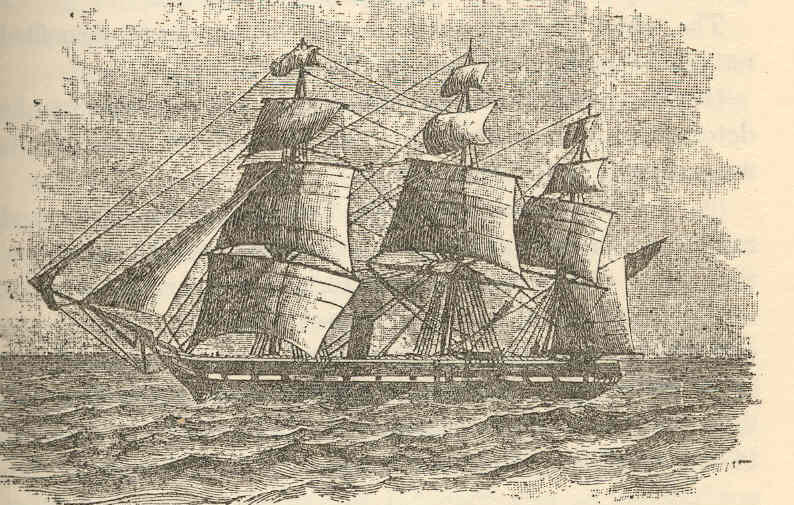
\includegraphics[width=0.55\linewidth]{images/book1/g8-challenger-sounding.jpg}

{\small HMS \emph{Challenger} 号准备测量\omterm{def:g2:water-on-earth:ocean}{海洋}深度，
1872 年。版画取自远征报告，转载于
W.~A.~Herdman, \emph{Founders of Oceanography}（1923）；公有领域，经
维基共享资源。}
% ledger: commons:challenger
\label{fig:g8:the-oceans:challenger}
\end{omfigure}

如今，船只用声音测绘海底。船底下方的一个装置
向下发出一个短促的声脉冲，声音碰到海底后反射
回来形成回声。回声往返所用的时间给出水深，
船只继续航行，不断测深。这就是\emph{声呐}。
% ledger: nos:sonar

\begin{recall}
\omterm{def:g2:water-on-earth:salt-fresh}{咸水}覆盖地球大部分表面，汇成一个世界大洋，
再划分为大洋和海（见\cref{ch:g2:water-on-earth}）。
板块在\omterm{def:g8:the-oceans:seafloor}{洋脊}处相互分离，一个板块在\omterm{def:g8:the-oceans:seafloor}{海沟}处俯冲
到另一板块之下（见\cref{ch:g7:plate-tectonics}）。\omterm{def:g2:water-on-earth:ocean}{海洋}上空，风沿着大范围的
带状区域吹送：\omterm{def:g8:winds-global-circulation:global-winds}{信风}、\omterm{def:g8:winds-global-circulation:global-winds}{西风带}与\omterm{def:g8:winds-global-circulation:global-winds}{极地东风带}，受
地球自转偏转（见\cref{ch:g8:winds-global-circulation}）。
\end{recall}

\section{海底}

如果把海水全部抽干，一整片隐藏的
\omterm{def:g1:landscapes-around-us:landscape}{景观}就会显现。沿\omterm{def:g1:landscapes-around-us:water}{海岸}，陆地延伸到海面下，
形成平缓的浅水陆架；随后海底沿着陡坡
下降，进入广阔、平坦而深达数千米的\omterm{def:g8:the-oceans:seafloor}{深海平原}。
\omterm{def:g1:landscapes-around-us:landform}{平原}之上耸立着\omterm{def:g4:world-physical-map:range}{山脉}，有时还有狭窄的
\omterm{def:g8:the-oceans:seafloor}{海沟}，深度超过地球上的其他任何地方。
% ledger: edin:challenger-stations

\begin{omfigure}
\begin{tikzpicture}[font=\footnotesize, >={Stealth[length=2mm]}]
  \fill[omSea] (0,0) rectangle (15.6,-4.2);
  \fill[omLithAlluv] (0,0.6) -- (1.2,0.15) -- (1.6,0) -- (3.4,-0.35)
    .. controls (3.9,-0.55) and (4.1,-2.6) .. (4.7,-3.1)
    -- (6.6,-3.35) -- (7.6,-3.1) -- (8.3,-2.2) -- (8.6,-1.7) -- (8.75,-1.9) -- (8.9,-1.65) -- (9.2,-2.3) -- (10.0,-3.15)
    -- (11.6,-3.4) -- (12.6,-3.45) -- (13.05,-4.1) -- (13.35,-3.0) -- (14.2,-0.9) -- (14.8,0.7) -- (15.6,1.3)
    -- (15.6,-4.6) -- (0,-4.6) -- cycle;
  \draw[black!70] (0,0.6) -- (1.2,0.15) -- (1.6,0) -- (3.4,-0.35)
    .. controls (3.9,-0.55) and (4.1,-2.6) .. (4.7,-3.1)
    -- (6.6,-3.35) -- (7.6,-3.1) -- (8.3,-2.2) -- (8.6,-1.7) -- (8.75,-1.9) -- (8.9,-1.65) -- (9.2,-2.3) -- (10.0,-3.15)
    -- (11.6,-3.4) -- (12.6,-3.45) -- (13.05,-4.1) -- (13.35,-3.0) -- (14.2,-0.9) -- (14.8,0.7) -- (15.6,1.3);
  \draw[omRiver] (1.55,0) -- (14.45,0);
  \node[anchor=south] at (8,0.05) {海平面};
  \node[align=center] at (2.6,-0.85) {大陆架};
  \draw[->] (2.6,-0.55) -- (2.6,-0.25);
  \node[align=center, anchor=east] at (3.7,-2.0) {大陆坡};
  \draw[->] (3.75,-2.0) -- (4.1,-1.9);
  \node[align=center] at (5.7,-2.6) {深海平原};
  \node[align=center] at (8.75,-0.9) {洋脊};
  \draw[->] (8.75,-1.15) -- (8.75,-1.55);
  \node[align=center] at (11.1,-2.6) {深海平原};
  \node[align=center, anchor=west] at (13.5,-3.9) {海沟};
  \draw[->] (13.45,-3.9) -- (13.15,-3.9);
  \node[anchor=south] at (0.8,0.6) {大陆};
  \node[anchor=south east] at (14.7,1.0) {山脉};
\end{tikzpicture}

{\small 海底各组成部分，从\omterm{def:g1:landscapes-around-us:water}{海岸}到远洋直至
另一侧\omterm{def:g1:landscapes-around-us:water}{海岸}（示意图，深度与宽度并非按比例绘制）。}
\label{fig:g8:the-oceans:sketch}
\end{omfigure}

\begin{definition}[海底的各个组成部分]\label{def:g8:the-oceans:seafloor}
\begin{itemize}
  \item \emph{大陆架}\index{大陆架}是
        \omterm{def:g3:continents-and-oceans:continent}{大陆}位于海面下的浅而平缓倾斜的边缘。
  \item \emph{大陆坡}\index{大陆坡}是
        从陆架通向深海海底的陡峭斜坡。
  \item \emph{深海平原}\index{深海平原}是
        广阔、非常平坦而深邃的海底部分。
  \item \emph{洋脊}\index{洋脊}是
        从深海\omterm{def:g1:landscapes-around-us:landform}{平原}上隆起的一长串水下\omterm{def:g4:world-physical-map:range}{山脉}。
  \item \emph{海沟}\index{海沟}是一条狭长而
        非常深的海底槽形凹陷，常靠近一列
        \omterm{def:g4:world-physical-map:range}{山脉}或\omterm{def:g4:volcanoes-earthquakes-first-look:volcano}{火山}岛链。
\end{itemize}
\end{definition}
% ledger: edin:challenger-stations, usgs:trench-depth

\omterm{def:g2:water-on-earth:ocean}{海洋}的平均深度约为 \qty{3700}{m}，几乎是
陆地上最高山峰高度的一半。其最深处是
太平洋马里亚纳\omterm{def:g8:the-oceans:seafloor}{海沟}中的挑战者深渊，
位于海面以下近 \qty{11000}{m}。
% ledger: nos:ocean-depth, usgs:trench-depth, tht:everest


\begin{method}[读取海底剖面图]
\begin{enumerate}
  \item 读取坐标轴：横向距离、向上的高度或向下的深度，以及
        竖向夸大倍数。
  \item 找出\omterm{def:g4:world-physical-map:altitude}{海平面}（高度为 0），并确定剖面与其相交的
        \omterm{def:g1:landscapes-around-us:water}{海岸}位置。
  \item 从\omterm{def:g1:landscapes-around-us:water}{海岸}出发沿海底观察：先是浅的\omterm{def:g8:the-oceans:seafloor}{大陆架}，接着是陡峭的
        \omterm{def:g8:the-oceans:seafloor}{大陆坡}，然后是深而平坦的\omterm{def:g8:the-oceans:seafloor}{深海平原}。
  \item 寻找从\omterm{def:g1:landscapes-around-us:landform}{平原}上隆起的部分（即\omterm{def:g8:the-oceans:seafloor}{洋脊}），或低于\omterm{def:g1:landscapes-around-us:landform}{平原}的部分
        （即\omterm{def:g8:the-oceans:seafloor}{海沟}），并读出其深度。
\end{enumerate}
\end{method}

\begin{example}[横跨南大西洋]
上方剖面图中，越过南美洲\omterm{def:g1:landscapes-around-us:water}{海岸}后，海底
在不到 \qty{300}{km} 的距离内，海底深度超过 \qty{3000}{m}。\omterm{def:g8:the-oceans:seafloor}{深海平原}的
深度介于 \qty{3500}{m} 与 \qty{5000}{m} 之间，几乎占据整个宽度。
大约在横跨途中，即沿剖面 \qty{4400}{km} 处，大西洋中脊
升至海面以下约 \qty{2300}{m}，比\omterm{def:g1:landscapes-around-us:landform}{平原}高出 \qty{2000}{m} 以上，
是一座隐藏在海下的\omterm{def:g4:world-physical-map:range}{山脉}。\omterm{def:g1:landscapes-around-us:landform}{平原}再次加深至
超过 \qty{5000}{m}，之后海底才向非洲一侧抬升。
\end{example}
% ledger: data:etopo1 (figdata/grade-8/seafloor_profile.py: ridge crest -2329 m at 4407 km; deepest -5295 m)

\begin{omfigure}
\begin{tikzpicture}
\begin{axis}[omsection, scale only axis, width=14cm, height=3.6cm, xmin=0, xmax=7569,
  ymin=-6000, ymax=1500, ytick={-6000,-4000,-2000,0}, xtick={0,1000,...,7000},
  xlabel={沿南纬 30.5\textdegree\ 的距离，自西经 59.5\textdegree\ 起 (km)}, ylabel={高度 (m)},
  tick label style={font=\scriptsize}, label style={font=\small},
  yticklabel style={/pgf/number format/1000 sep={\,}}, xticklabel style={/pgf/number format/1000 sep={\,}},
  axis background/.style={fill=white}, clip=true]
  \fill[omSea] (axis cs:0,-6000) rectangle (axis cs:7569,0);
  \addplot[fill=omLithAlluv, draw=black!70, line width=0.5pt] table[x=km, y=elev_m] {figdata/out/grade-8-seafloor_profile-atlantic-rock.dat};
  \node[font=\scriptsize, align=center, fill=white, inner sep=1pt] at (axis cs:4407,-900) {大西洋中脊};
  \draw[-{Stealth[length=1.5mm]}] (axis cs:4407,-1250) -- (axis cs:4407,-2150);
  \node[font=\scriptsize] at (axis cs:2500,-5300) {深海平原};
  \node[font=\scriptsize] at (axis cs:6200,-5600) {深海平原};
  \node[font=\scriptsize, anchor=south west] at (axis cs:30,350) {南美洲};
  \node[font=\scriptsize, anchor=south east] at (axis cs:7380,350) {非洲};
  \node[anchor=north] at (rel axis cs:0.75,0.97) {\omve{260}};
\end{axis}
\end{tikzpicture}

\medskip
\begin{tikzpicture}
\begin{axis}[omsection, scale only axis, width=7cm, height=3.6cm, xmin=0, xmax=3020,
  ymin=-6000, ymax=4500, ytick={-6000,-4000,-2000,0,2000,4000}, xtick={0,1000,2000,3000},
  xlabel={沿南纬 20.5\textdegree\ 的距离 (km)}, ylabel={高度 (m)},
  tick label style={font=\scriptsize}, label style={font=\small},
  yticklabel style={/pgf/number format/1000 sep={\,}}, xticklabel style={/pgf/number format/1000 sep={\,}},
  axis background/.style={fill=white}, clip=true]
  \fill[omSea] (axis cs:0,-6000) rectangle (axis cs:3020,0);
  \addplot[fill=omLithAlluv, draw=black!70, line width=0.5pt] table[x=km, y=elev_m] {figdata/out/grade-8-seafloor_profile-pacific-rock.dat};
  \node[font=\scriptsize, align=center, fill=white, inner sep=1pt] at (axis cs:1300,1600) {秘鲁–智利海沟};
  \draw[-{Stealth[length=1.5mm]}] (axis cs:1750,1150) -- (axis cs:1870,-5000);
  \node[font=\scriptsize, anchor=west] at (axis cs:2600,3500) {安第斯山脉};
  \node[font=\scriptsize] at (axis cs:700,-5300) {深海平原};
  \node[anchor=north west] at (rel axis cs:0.01,0.98) {\omve{148}};
\end{axis}
\end{tikzpicture}

{\small 两幅真实海底剖面图，数据取自 ETOPO1 地形数据，
每隔一度\omterm{def:g6:latitude-longitude:longitude}{经度}取一个点。上图：横跨南大西洋，自南美洲
至非洲。下图：横跨南美洲太平洋一侧。
图中高度相对于距离分别被放大 260 倍和 148 倍
（\emph{竖向夸大}），否则\omterm{def:g2:water-on-earth:ocean}{海洋}看起来会薄得像
一张纸；由于每一度只取一个点，狭窄的\omterm{def:g8:the-oceans:seafloor}{海沟}看起来
比实际要浅。}
% ledger: data:etopo1, earth:Rmean (figdata/grade-8/seafloor_profile.py)
\label{fig:g8:the-oceans:profiles}
\end{omfigure}


\section{咸水}

海水尝起来是咸的，因为其中溶有盐分。其中大部分
来自\omterm{def:g3:continents-and-oceans:continent}{大陆}的\omterm{def:g3:stones-pebbles-sand:rock}{岩石}：雨水缓慢\omterm{def:g5:water-shapes-the-land:erosion}{侵蚀}\omterm{def:g3:stones-pebbles-sand:rock}{岩石}，
\omterm{def:g1:landscapes-around-us:water}{河流}将溶解的盐分带入大海。还有一部分来自
海底的热泉。
% ledger: nos:salinity-varies

\begin{definition}[盐度]\label{def:g8:the-oceans:salinity}
海水的\emph{盐度}\index{盐度}，是指每千克海水中溶解的
盐类质量。平均每千克约为
\qty{35}{g}，即海水质量的 \qty{3.5}{\%}
为盐。
\end{definition}
% ledger: nos:salinity-varies

\omterm{def:g8:the-oceans:salinity}{盐度}并非处处相同。海水蒸发时，水分逸散而盐分
留在水中：太阳照射强烈、降雨稀少的地方，
海水变得更咸。降雨丰沛，或有大河
汇入的地方，海水则较淡。海水凝固成
海冰时，盐分留在周围的水中，使其也变得更咸。
总体而言，\omterm{def:g3:continents-and-oceans:equator}{赤道}附近降雨丰富，\omterm{def:g8:the-oceans:salinity}{盐度}较低，
极地附近亦较低；\omterm{def:g8:the-oceans:salinity}{盐度}最高的是中\omterm{def:g6:latitude-longitude:latitude}{纬度}地区，
即 \ang{30} 附近的\omterm{def:g5:natural-hazards:drought}{干旱}带下方。
% ledger: nos:salinity-varies, nos:sea-ice-salt, mo:three-cells

\begin{omfigure}
\begin{tikzpicture}[font=\footnotesize, >={Stealth[length=2mm]}]
  \fill[omSea] (0,0) rectangle (13,-1.6);
  \draw[omRiver, line width=0.8pt] (0,0) -- (13,0);
  % left: dry belt, evaporation
  \fill[yellow!80!orange] (1.2,3.0) circle (0.35);
  \foreach \x in {1.0,1.8,2.6,3.4} \draw[->, black!50, line width=0.9pt, decorate, decoration={snake, amplitude=0.6mm, segment length=3mm}] (\x,0.15) -- (\x,1.6);
  \node[align=center] at (2.3,2.2) {强烈蒸发，\\雨水稀少};
  \node[align=center, fill=white, inner sep=1.5pt] at (2.3,-0.8) {\textbf{更咸}};
  % middle: rain
  \fill[black!20] (5.2,2.9) ellipse [x radius=1.3, y radius=0.4];
  \foreach \x in {4.4,4.8,...,6.0} \draw[omRiver] (\x,2.45) -- (\x-0.2,0.25);
  \node[align=center, fill=white, inner sep=1.5pt] at (5.2,-0.8) {\textbf{较淡}};
  \node at (5.2,3.55) {大雨};
  % right: river mouth and sea ice
  \fill[omLithAlluv] (7.4,0) -- (9.6,0) -- (9.6,0.6) -- (7.4,0.35) -- cycle;
  \draw[omRiver, line width=2pt, ->] (9.4,0.45) -- (7.9,0.2);
  \node[anchor=south] at (8.6,0.65) {河流};
  \node[align=center, fill=white, inner sep=1.5pt] at (8.6,-0.8) {\textbf{较淡}};
  \fill[white, draw=omCold] (10.6,0.25) -- (12.6,0.25) -- (12.4,-0.25) -- (10.8,-0.25) -- cycle;
  \node[anchor=south] at (11.6,0.3) {海冰形成};
  \node[align=center, fill=white, inner sep=1.5pt] at (11.6,-0.95) {\textbf{更咸}\\（盐分残留）};
\end{tikzpicture}

{\small 改变海水\omterm{def:g8:the-oceans:salinity}{盐度}的因素：蒸发和结冰使盐分留下，
降雨和\omterm{def:g1:landscapes-around-us:water}{河流}则带来\omterm{def:g2:water-on-earth:salt-fresh}{淡水}。}
% ledger: nos:salinity-varies, nos:sea-ice-salt
\label{fig:g8:the-oceans:salinity}
\end{omfigure}

\begin{omfigure}
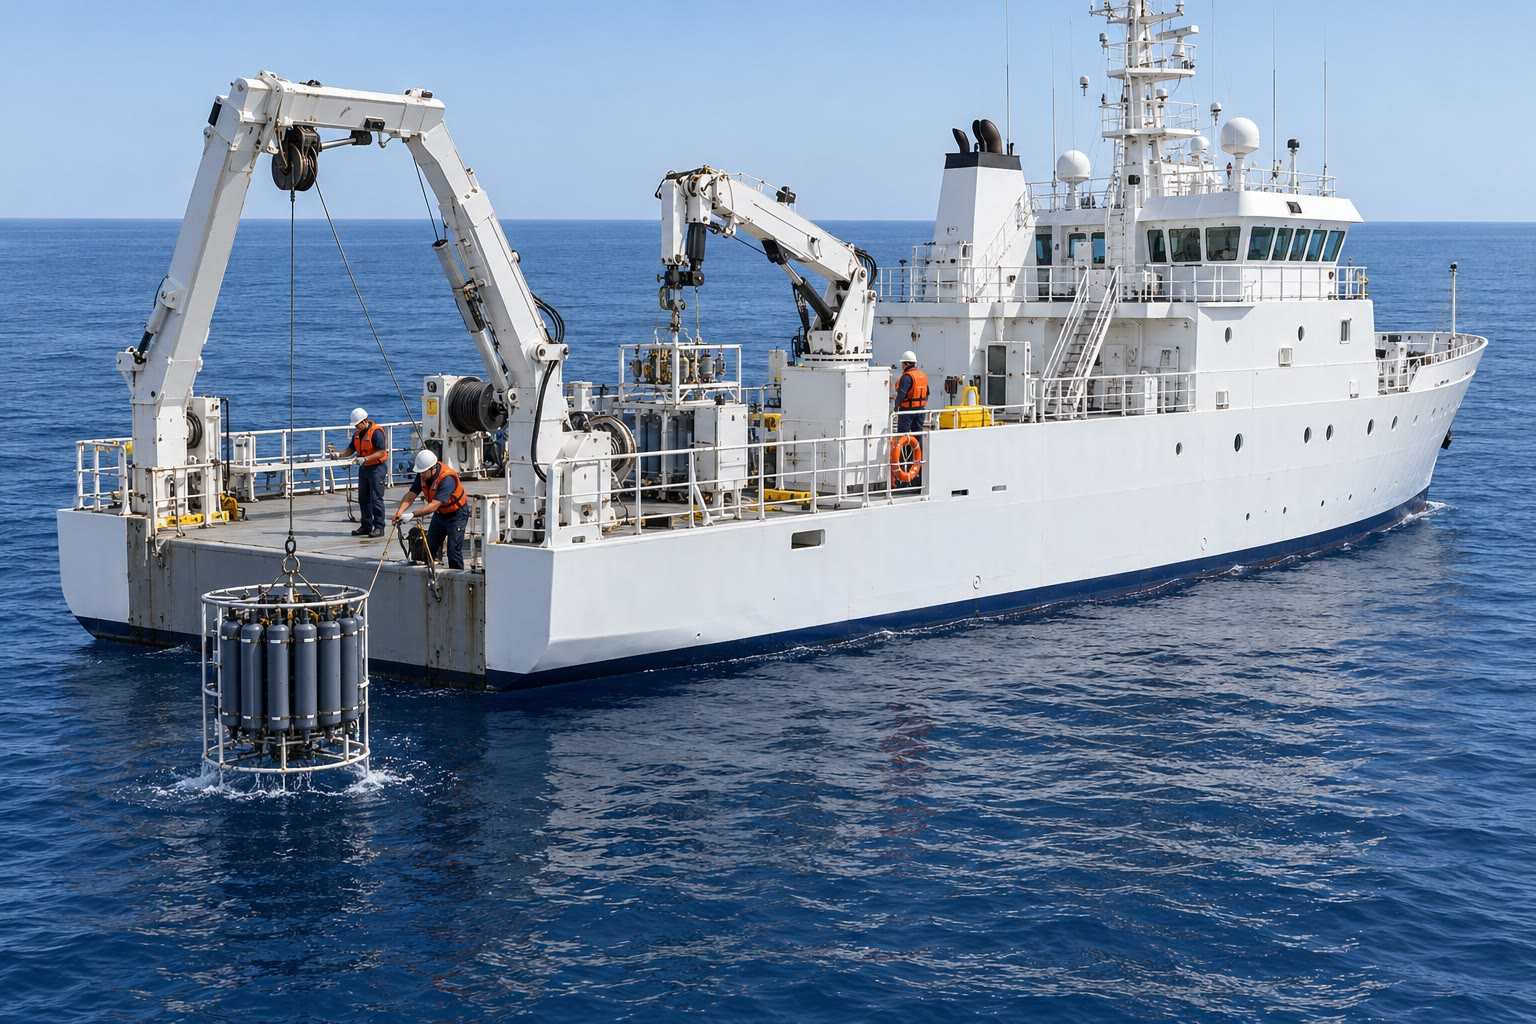
\includegraphics[width=0.58\linewidth]{images/book1/ai/g8-research-ship.jpg}

{\small 一艘科考船将装有采样瓶的框架放入海中，
以取回深层海水，并测量其\omterm{def:g8:the-oceans:salinity}{盐度}和
温度（通用场景的 AI 生成插图）。}
\label{fig:g8:the-oceans:ship}
\end{omfigure}

\section{表层洋流}

\omterm{def:g2:water-on-earth:ocean}{海洋}从不静止。风拖拽海面，使海水运动：
稳定的\omterm{def:g8:winds-global-circulation:global-winds}{信风}在\omterm{def:g3:continents-and-oceans:equator}{赤道}附近推动海水向西流动，
\omterm{def:g8:winds-global-circulation:global-winds}{西风带}则在中\omterm{def:g6:latitude-longitude:latitude}{纬度}推动海水向东流动。
与风一样，运动的海水也受地球自转影响而偏转：
在\omterm{def:g3:continents-and-oceans:equator}{北半球}向右偏，
在\omterm{def:g3:continents-and-oceans:equator}{南半球}向左偏。
% ledger: nos:gyres

\begin{definition}[洋流与环流]\label{def:g8:the-oceans:current}
\emph{洋流}\index{洋流}是海水沿某一方向的稳定运动，
如同\omterm{def:g2:water-on-earth:ocean}{海洋}中的\omterm{def:g1:landscapes-around-us:water}{河流}。
\emph{环流}\index{环流}是由洋流构成的巨大环路，
绕洋盆回转。
\end{definition}
% ledger: nos:gyre-def, nos:gyres
\phantomsection\label{def:g8:the-oceans:gyre}

全球共有五大\omterm{def:g8:the-oceans:current}{环流}：北大西洋和南大西洋、北太平洋和南太平洋，
以及印度洋。\omterm{def:g3:continents-and-oceans:equator}{北半球}的\omterm{def:g8:the-oceans:current}{环流}沿顺时针方向转动，
\omterm{def:g3:continents-and-oceans:equator}{南半球}的\omterm{def:g8:the-oceans:current}{环流}则沿逆时针方向转动。
在每个大洋的西侧，\omterm{def:g8:the-oceans:current}{环流}的\omterm{def:g8:the-oceans:current}{洋流}狭窄而快速；
在东侧，则宽阔而缓慢。
% ledger: nos:gyres

\begin{inthelab}[盘中的环流]
在室内，往一个大圆盘中注入清水，在水面撒一小撮胡椒粉。
用吸管贴近盘子的一侧，沿同一方向平稳地轻吹。
观察胡椒粉：靠近水面的水随着吹气开始流动，
不久，水面便随之流动，
整个水面绕着圆盘形成一个\omterm{def:g8:the-oceans:current}{环流}。
\end{inthelab}

\begin{omfigure}
\begin{tikzpicture}
\begin{axis}[ommap, width=\linewidth, xmin=-180, xmax=180, ymin=-65, ymax=70,
  xtick={-180,-120,...,180}, ytick={-60,-30,0,30,60},
  xticklabels={$180^\circ$,$120^\circ$西, $60^\circ$西, $0^\circ$,$60^\circ$东, $120^\circ$东, $180^\circ$},
  yticklabels={$60^\circ$南, $30^\circ$南, $0^\circ$,$30^\circ$北, $60^\circ$北},
  tick label style={font=\scriptsize}]
  \addplot[fill=omLithAlluv, draw=black!45, line width=0.2pt] table {figdata/out/shared-geo-land.dat};
  \addplot[omWarm, line width=1.3pt] table {figdata/out/grade-8-ocean_currents-gyres-warm.dat};
  \addplot[omCold, line width=1.3pt] table {figdata/out/grade-8-ocean_currents-gyres-cold.dat};
  \addplot[quiver={u=\thisrow{u}, v=\thisrow{v}}, -{Stealth[length=2.6mm, width=2.2mm]}, omWarm, line width=1.3pt]
    table[x=lon, y=lat] {figdata/out/grade-8-ocean_currents-heads-warm.dat};
  \addplot[quiver={u=\thisrow{u}, v=\thisrow{v}}, -{Stealth[length=2.6mm, width=2.2mm]}, omCold, line width=1.3pt]
    table[x=lon, y=lat] {figdata/out/grade-8-ocean_currents-heads-cold.dat};
  \node[font=\scriptsize\bfseries, fill=white, inner sep=1pt, anchor=east] at (axis cs:-72,40) {墨西哥湾流};
  \node[font=\scriptsize\bfseries, fill=white, inner sep=1pt, anchor=west] at (axis cs:-12,25) {加那利洋流};
\end{axis}
\end{tikzpicture}

{\small 五大\omterm{def:g8:the-oceans:current}{环流}简图：\omterm{def:g3:continents-and-oceans:equator}{北半球}顺时针，\omterm{def:g3:continents-and-oceans:equator}{南半球}逆时针。
红色：暖流，来自热带。
蓝色：寒流，来自较高\omterm{def:g6:latitude-longitude:latitude}{纬度}。
北大西洋\omterm{def:g8:the-oceans:current}{环流}的西侧以墨西哥湾流为界，
东侧以加那利\omterm{def:g8:the-oceans:current}{洋流}为界。}
% ledger: nos:gyres, data:ne-land (figdata/grade-8/ocean_currents.py)
\label{fig:g8:the-oceans:gyres}
\end{omfigure}

这些\omterm{def:g8:the-oceans:current}{洋流}中最著名的是墨西哥湾流。它从墨西哥湾
流出，沿佛罗里达\omterm{def:g1:landscapes-around-us:water}{海岸}向北，在北卡罗来纳州外海转向东，
然后向东北方向横穿大西洋。其暖水
平均流速约为 \qty{6.4}{km} 每小时，
表层流速最高可达约 \qty{9}{km} 每小时，
其输送的水量超过世界上所有\omterm{def:g1:landscapes-around-us:water}{河流}的总和。
它使佛罗里达东\omterm{def:g1:landscapes-around-us:water}{海岸}冬季更温暖，并为西欧带来温和的空气。
% ledger: nos:gulf-stream, nos:gyres

\begin{omfigure}
\begin{minipage}[c]{0.5\linewidth}\centering
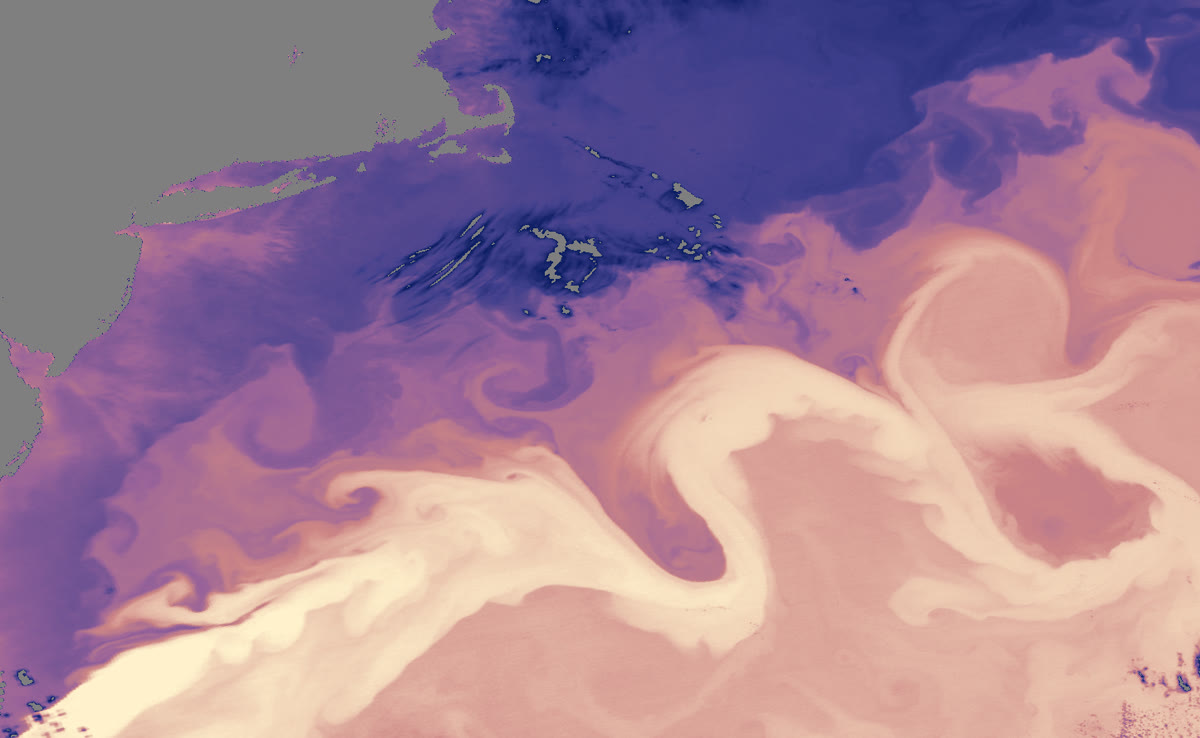
\includegraphics[width=\linewidth]{images/book1/g8-gulf-stream-sst.jpg}
\end{minipage}\hfill
\begin{minipage}[c]{0.46\linewidth}\raggedright
{\small 2005 年 4 月 18 日，美国国家航空航天局（NASA）的 Aqua 卫星
测得的北美东\omterm{def:g1:landscapes-around-us:water}{海岸}外海表温度。墨西哥湾流是
一条暖水带（颜色较浅，最高约 \qty{23}{\degreeCelsius}），
自左下方向右蜿蜒延伸，
两侧是较冷的海水（颜色较深，最低约 \qty{-1}{\degreeCelsius}），
陆地为灰色。
NASA（公有领域，经由维基共享资源）。}
\end{minipage}
% ledger: commons:gulf-sst
\label{fig:g8:the-oceans:gulf}
\end{omfigure}


\section{深层洋流与海洋热量}

风驱动表层\omterm{def:g8:the-oceans:current}{洋流}。在深处，即寒冷幽暗的深海中，
海水同样在流动，只是慢得多。
在遥远的北大西洋，墨西哥湾流带来的暖水把热量传给寒冷的空气；
水变冷后，若形成海冰，盐分会留下，使海水变咸，密度增大，
并下沉至海底。这股冷而咸的海水沿海底向南爬行，
一直到达\omterm{def:g3:continents-and-oceans:poles}{南极}洲，然后进入印度洋和太平洋，
在那里缓慢上升并回到表层。一滴水完成这一巨大\omterm{def:g8:the-oceans:current}{环流}
大约需要 \num{1000} 年，
这就是\emph{全球\omterm{def:g8:the-oceans:current}{洋流}传送带}。
% ledger: nos:conveyor, nos:sea-ice-salt

\begin{omfigure}
\begin{tikzpicture}
\begin{axis}[ommap, width=\linewidth, xmin=-180, xmax=180, ymin=-65, ymax=70,
  xtick={-180,-120,...,180}, ytick={-60,-30,0,30,60},
  xticklabels={$180^\circ$,$120^\circ$西, $60^\circ$西, $0^\circ$,$60^\circ$东, $120^\circ$东, $180^\circ$},
  yticklabels={$60^\circ$南, $30^\circ$南, $0^\circ$,$30^\circ$北, $60^\circ$北},
  tick label style={font=\scriptsize}]
  \addplot[fill=omLithAlluv, draw=black!45, line width=0.2pt] table {figdata/out/shared-geo-land.dat};
  \addplot[omWarm, line width=1.3pt] table {figdata/out/grade-8-conveyor-surface.dat};
  \addplot[omCold, line width=1.3pt, dashed] table {figdata/out/grade-8-conveyor-deep.dat};
  \addplot[quiver={u=\thisrow{u}, v=\thisrow{v}}, -{Stealth[length=2.6mm, width=2.2mm]}, omWarm, line width=1.3pt]
    table[x=lon, y=lat] {figdata/out/grade-8-conveyor-heads-surface.dat};
  \addplot[quiver={u=\thisrow{u}, v=\thisrow{v}}, -{Stealth[length=2.6mm, width=2.2mm]}, omCold, line width=1.3pt]
    table[x=lon, y=lat] {figdata/out/grade-8-conveyor-heads-deep.dat};
  \node[font=\scriptsize\bfseries, fill=white, inner sep=1pt, anchor=west] at (axis cs:4,64) {下沉};
  \node[font=\scriptsize\bfseries, fill=white, inner sep=1pt, anchor=south] at (axis cs:163,11) {上升};
\end{axis}
\end{tikzpicture}

{\small 全球\omterm{def:g8:the-oceans:current}{洋流}传送带，简化为单一\omterm{def:g8:the-oceans:current}{环流}（示
意图）。红色：表层暖水；蓝色虚线：冷而咸的海水
沿深海海底爬行。海水在遥远的北大西洋下沉
，位于格陵兰与挪威之间，并在太平洋（以及
图中未画出的印度洋）上升。}
% ledger: nos:conveyor, data:ne-land (figdata/grade-8/conveyor.py)
\end{omfigure}

\begin{example}[深层海水有多慢？]\label{ex:g8:the-oceans:deep-speed}
图上所示的\omterm{def:g8:the-oceans:current}{环流}大约长 \qty{70000}{km}。若一滴水
绕行一周约需 \num{1000} 年，则其平均速率约为
$\num{70000} \div \num{1000} = \qty{70}{km}$ 每年，即
每天约 \qty{200}{m}。墨西哥湾流以每小时 \qty{6.4}{km} 的速度，
一天约流过 \qty{150}{km}：仅约 11 小时，
便可走完深层海水整整一年所走的距离。
% ledger: nos:conveyor, nos:gulf-stream, earth:Rmean (loop length and speeds computed in figdata/grade-8/conveyor.py)
\end{example}

表层与深层\omterm{def:g8:the-oceans:current}{洋流}共同输送热量：暖水自
热带流向两极，冷水则流回
\omterm{def:g3:continents-and-oceans:equator}{赤道}。与风一样，\omterm{def:g2:water-on-earth:ocean}{海洋}也在调节太阳对地球的
不均匀加热。
% ledger: nos:conveyor, nos:gulf-stream, mo:global-circ

\section{练习}

\begin{exercise}[$\star$]\label{exo:g8:the-oceans:1}
请将下列海底地形按潜艇驶离\omterm{def:g1:landscapes-around-us:water}{海岸}、前往大西洋中部时
依次遇到的顺序排列：\omterm{def:g8:the-oceans:seafloor}{深海平原}；
\omterm{def:g8:the-oceans:seafloor}{大陆坡}；\omterm{def:g8:the-oceans:seafloor}{洋脊}；\omterm{def:g8:the-oceans:seafloor}{大陆架}。
\end{exercise}

\begin{exercise}[$\star$]\label{exo:g8:the-oceans:2}
判断下列句子的对错，并改正错误的句子。(a) \omterm{def:g2:water-on-earth:ocean}{海洋}的平均深度约为
\qty{37}{km}。(b) \omterm{def:g3:continents-and-oceans:equator}{北半球}的\omterm{def:g8:the-oceans:current}{环流}
顺时针旋转。(c) 蒸发使海水变得不那么咸。(d) 墨西哥湾
流是一股暖流。
\end{exercise}

\begin{exercise}[$\star$]\label{exo:g8:the-oceans:3}
写出与下列每项描述对应的词：(a) 海底下方的
长链状\omterm{def:g4:world-physical-map:range}{山脉}；(b) 每千克海水中盐的质量；(c) 一个非常巨大的
\omterm{def:g8:the-oceans:current}{洋流}环路；(d) 海底中一条狭长而极深的
\omterm{def:g8:the-oceans:seafloor}{海沟}。
\end{exercise}

\begin{exercise}[$\star$]\label{exo:g8:the-oceans:4}
根据\omterm{def:g8:the-oceans:current}{环流}图：(a) 南大西洋的\omterm{def:g8:the-oceans:current}{环流}
向哪个方向旋转？(b) 说出北大西洋中的一股暖流和一股冷流的名称。
(c) \omterm{def:g3:continents-and-oceans:equator}{赤道}附近哪些风把海水推向西方？
\end{exercise}

\begin{exercise}[$\star\star$]\label{exo:g8:the-oceans:5}
取 \qty{1}{kg} 海水样品，其中含有 \qty{35}{g} 盐分。(a)
样品中盐分的质量占其质量的百分之几？(b) 在 \qty{20}{kg} 这种海水中，
共有多少克盐分？(c) 多少千克海水
含有 \qty{1}{kg} 盐分？
\end{exercise}

\begin{exercise}[$\star\star$]\label{exo:g8:the-oceans:6}
一艘船的声呐竖直向下发出一个声脉冲，回声
在 \qty{6}{s} 后返回。声音在海水中每秒约传播
\qty{1500}{m}。(a) 声音在 \qty{6}{s} 内传播了多远？(b) 为什么
深度只是这段距离的一半？(c) 水深是多少？(d) 船可能位于
海底的哪个部分上方？
\end{exercise}

\begin{exercise}[$\star\star$]\label{exo:g8:the-oceans:7}
利用南大西洋的剖面图。(a) \omterm{def:g8:the-oceans:seafloor}{深海平
原}大约深多少？(b) 沿剖面的哪一距离处是
大西洋中脊的脊顶，其深度是多少？(c) 脊顶
比\omterm{def:g1:landscapes-around-us:landform}{平原}高出多少米？(d) 为什么剖面图需要
竖向夸大？
\end{exercise}

\begin{exercise}[$\star\star$]\label{exo:g8:the-oceans:8}
甲海位于两片\omterm{def:g5:weather-and-climate:desert}{沙漠}之间：那里几乎从不下雨，且没有大
河注入。乙海位于多雨地区，接纳许多大河。
试解释哪一片海比大洋更咸，哪一片
比大洋更淡。请使用词语\emph{蒸发}、\emph{\omterm{def:g2:water-on-earth:salt-fresh}{淡水}}、\emph{盐
分留下}。
\end{exercise}

\begin{exercise}[$\star\star$]\label{exo:g8:the-oceans:9}
一只漂流瓶在佛罗里达\omterm{def:g1:landscapes-around-us:water}{海岸}外被投入大海。
(a) 最先由哪股\omterm{def:g8:the-oceans:current}{洋流}带着它漂流，朝哪个方向？(b) 随后它朝
哪个方向穿越大西洋？(c) 若它继续沿\omterm{def:g8:the-oceans:current}{环流}绕行，
它会沿哪一\omterm{def:g1:landscapes-around-us:water}{海岸}向南行进？(d) 这股\omterm{def:g8:the-oceans:current}{洋流}是暖流还是冷流？
\end{exercise}

\begin{exercise}[$\star\star$]\label{exo:g8:the-oceans:10}
墨西哥湾流的平均流速约为每小时 \qty{6.4}{km}。(a) 其水流一天
能流过多远？(b) 一周呢？(c) 与一名步行速度为
每小时 \qty{5}{km} 的人相比。
\end{exercise}

\begin{exercise}[$\star\star\star$]\label{exo:g8:the-oceans:11}
\omterm{def:g2:water-on-earth:ocean}{海洋}的平均深度约为 \qty{3700}{m}，
最深处的深度接近 \qty{11000}{m}。
(a) 将两个深度都换算为千米。(b) 最深处比平均深度深多少倍？结果保留一位小数。
(c) 从最深处反射回来的声呐回声，
以每秒 \qty{1500}{m} 计，需要多少秒才能返回？(d) 北大西洋中，
一滴水沿“传送带”下沉。
若绕行一周约需\num{1000} 年，用 10 的幂次表示这是多少年。
\end{exercise}

\begin{exercise}[$\star\star\star$]\label{exo:g8:the-oceans:12}
深海的大“传送带”始于挪威海，位于挪威\omterm{def:g1:landscapes-around-us:water}{海岸}外，
那里由墨西哥湾流带来的暖水将热量传给冷空气。
(a) 利用\omterm{def:g8:the-oceans:current}{洋流}\omterm{def:g8:the-oceans:current}{环流}图和本章内容，
逐步说明这股暖水如何从热带流到那里，
以及是哪些风推动了它。(b) 解释此后海水为何下沉。
(c) 接下来它流向何方？
\end{exercise}

\section{问题：漂流浮标}

\begin{problem}[{周末问题——一只漂流浮标在佛罗里达外海被投放，
并随北大西洋环流漂流；本题逐段追踪它的航程，
并计算它绕行一周所需的时间}]
\label{pb:g8:the-oceans:1}
% ledger: nos:drifter, nos:gulf-stream, nos:gyres (figdata/grade-8/ocean_currents.py; the leg lengths are rounded, the speeds of legs B to D are exercise data)
科学家在佛罗里达\omterm{def:g1:landscapes-around-us:water}{海岸}外投放一只漂流浮标。
它漂浮在略低于水面的位置，随\omterm{def:g8:the-oceans:current}{洋流}移动，
并将其位置发送给卫星。其电池约可使用一年。
图中显示了它绕北大西洋\omterm{def:g8:the-oceans:current}{环流}航行的四段路程。

\begin{center}
\begin{tikzpicture}
\begin{axis}[ommap, width=11.5cm, xmin=-95, xmax=0, ymin=5, ymax=55,
  xtick={-90,-60,-30,0}, ytick={10,30,50},
  xticklabels={$90^\circ$W,$60^\circ$W,$30^\circ$W,$0^\circ$},
  yticklabels={$10^\circ$N,$30^\circ$N,$50^\circ$N},
  tick label style={font=\scriptsize}]
  \addplot[fill=omLithAlluv, draw=black!45, line width=0.2pt] table {figdata/out/shared-geo-land.dat};
  \addplot[black, line width=1pt, densely dashed, postaction={decorate, decoration={markings,
      mark=between positions 0.04 and 0.98 step 0.08 with {\arrow{Stealth[length=2mm]}}}}]
    table[x=lon, y=lat] {figdata/out/grade-8-ocean_currents-buoy.dat};
  \addplot[only marks, mark=*, mark size=2.2pt, omDef] coordinates {(-79.5,26)};
  \node[font=\scriptsize\bfseries, anchor=east, fill=white, inner sep=1pt] at (axis cs:-81,26) {投放点};
  \addplot[only marks, mark=none, point meta=explicit symbolic, opacity=0, forget plot]
    table[x=lon, y=lat, meta=name] {figdata/out/grade-8-ocean_currents-buoy-legs.dat};
  \node[anchor=center, font=\footnotesize\bfseries, circle, fill=white, draw, inner sep=1pt] at (axis cs:-70,38) {A};
  \node[anchor=center, font=\footnotesize\bfseries, circle, fill=white, draw, inner sep=1pt] at (axis cs:-32,44.5) {B};
  \node[anchor=center, font=\footnotesize\bfseries, circle, fill=white, draw, inner sep=1pt] at (axis cs:-17,30.5) {C};
  \node[anchor=center, font=\footnotesize\bfseries, circle, fill=white, draw, inner sep=1pt] at (axis cs:-62,17) {D};
\end{axis}
\end{tikzpicture}

\medskip
{\small
\begin{tabular}{|c|l|c|c|}
\hline
航段 & \omterm{def:g8:the-oceans:current}{洋流} & 长度 (km) & 平均速率 （km/天） \\
\hline
A & 墨西哥湾流 & 3800 & 100 \\
B & 北大西洋暖流 & 2100 & 20 \\
C & 加那利寒流 & 3100 & 20 \\
D & 北\omterm{def:g3:continents-and-oceans:equator}{赤道}流 & 6100 & 20 \\
\hline
\end{tabular}}
\end{center}

\noindent\textbf{第一部分——投放。}\par\nopagebreak
\begin{enumerate}[beginpenalty=10000]
  \item 浮标在哪个大洋、哪个\omterm{def:g3:continents-and-oceans:equator}{半球}投放？
  \item \omterm{def:g8:the-oceans:current}{环流}沿哪个方向转动？浮标起初是被带向北方
        还是南方？
  \item 航段 A 的水是暖流还是冷流？航段 C 呢？请说明理由。
  \item 哪些风驱动航段 B 的\omterm{def:g8:the-oceans:current}{洋流}？航段 D 呢？
\end{enumerate}

\noindent\textbf{第二部分——绕行\omterm{def:g8:the-oceans:current}{环流}。}\par\nopagebreak
\begin{enumerate}[resume, beginpenalty=10000]
  \item 航段 A 需要多少天？
  \item 航段 B、C 和 D 各需要多少天？
  \item 绕行\omterm{def:g8:the-oceans:current}{环流}一周的总长度是多少？
  \item 为什么航段 A 比其他航段快得多？
\end{enumerate}

\noindent\textbf{第三部分——航程的长度。}\par\nopagebreak
\begin{enumerate}[resume, beginpenalty=10000]
  \item 浮标绕\omterm{def:g8:the-oceans:current}{环流}一周需要多少天？
  \item 若按 30 天为一个月计算，这相当于多少个月？结果四舍五入到
        最接近的整数月。
  \item 大约一年（365 天）后，电池会在
        哪一段航程耗尽？
  \item 若要让浮标把位置发回一整圈，
        电池还需多用几个月？
\end{enumerate}
\end{problem}
